\chapter{Einf\"uhrung in die Optimierung}

\section{Grundlagen}

\begin{Definition}
	\begin{center}
	Ein (mathematisches) \textbf {Optimierungsproblem}\index{allgemeines Optimierungssystem} hat die folgende Form\\
	\begin{gather}
  		\label{eq:P}   
  		\tag{P}
  			\begin{aligned}
    			\min_x
    			& & & f(x) \\
    			\text{s.t.}
    			& & & x\in \mathcal{F}
  			\end{aligned}
	\end{gather}
	\begin{itemize}
		\item  	$x=(x_1,\cdots,x_n)\tr\in\R^n$ sind die \textbf{Variablen}
		\item	$f\colon D\to\R, D\subset\R^n$, ist die \textbf{Zielfunktion}
		\item	$\mathcal{F}$ ist die \textbf{zul\"assige Menge}; ihre Elemente hei\ss en \textbf{zul\"assige Punkte}\qedhere
\end{itemize}
\end{center}
\end{Definition}

\paragraph{Die Nebenbedingungen}


\begin{itemize}
\item  Ist $\mathcal{F}=D$, dann spricht man von einem \textbf{unrestringierten Problem}.
\item Wird $\mathcal{F}$ durch Nebenbedingungen (Restiktionen) definiert, dann hei\ss t \eqref{eq:P} \textbf{restringiertes Optimierungsproblem} oder \textbf{Optimierungsproblem mit Nebenbedingungen}; $\mathcal{F}$ ist hierbei typischerweise durch Gleichungen und Ungleichungen definiert:
\begin{equation*}
	\mathcal{F}=\{x\in\R^n \mid h(x)=0,~ g(x)\leq 0\}
\end{equation*}

\paragraph{Einfache Beispiele}


\begin{enumerate}[label=\emph{\alph*})]
\item Mit $\mathcal{F}=D=\R$ sei $f\colon \R\to\R$ durch $f(x)=x^2$ definiert. Dann ist $x^\ast = 0$ die eindeutig bestimmte L\"osung von \eqref{eq:P}.
\item Mit $\mathcal{F}=D=\R$ sei $f\colon \R\to\R$ durch $f(x)=\sin(x)$ definiert. Dann hat \eqref{eq:P} unendlich viele L\"osungen $x^\ast=2k \pi-\frac{\pi}{2} ,k\in \mathbb{Z}$.
\item Mit $\mathcal{F}=D=\R$ sei $f\colon \R\to\R$ durch $f(x)=x$ definiert. In diesem Fall ist $f$ auf $\mathcal{F}$ nicht nach unten beschr\"ankt und \eqref{eq:P} hat keine L\"osung.
\item Mit $\mathcal{F}=D=\R$ sei $f\colon \R\to\R$ durch
\begin{equation*}
	f(x)= (2x-2)^2(3x+3)^2+10x
\end{equation*}
definiert. Dann ist der Punkt $x^\ast = -1$ globale L\"osung von \eqref{eq:P}. Der Punkt $\tilde{x}=1$ ist eine lokale L\"osung.
\item Wir betrachten das Problem
	\begin{gather}
	\label{eq:P2}   
	\tag{P2}
	\begin{aligned}
	\min_x
	& & & f(x) = x^3\\
	\text{s.t.}
	& & & x\geq 1
	\end{aligned}
	\end{gather}
Hier ist $D=\R$ und $\mathcal{F}=\{x\in\R \mid x\geq1 \}$. Der Punkt $x^\ast = 1$ ist L\"osung. Ohne die Restriktion h\"atte das Problem \eqref{eq:P2} keine L\"osung.
\end{enumerate}
\end{itemize}

\begin{Definition}(lokaler Minimalpunkt)~ \\
	Ein Punkt $x^\ast\in\F$ hei\ss t \textbf{lokaler Minimalpunkt} von $f$ auf $\F$ oder \textbf{lokale L\"osung} von \eqref{eq:P}, falls es ein $r>0$ mit
	\begin{equation*}
		f(x)\geq f(x^\ast) \qquad \forall x\in\F \cap B(x^\ast,r)
	\end{equation*}
	gibt. \vspace{5pt}\\
	Ein Punkt $x^\ast\in\F$ hei\ss t \textbf{strikter lokaler Minimalpunkt} von $f$ auf $\F$ oder \textbf{strikte lokale L\"osung} von \eqref{eq:P}, falls es ein $r>0$ mit
	\begin{equation*}
	f(x)> f(x^\ast) \qquad \forall x\in\F \cap B(x^\ast,r),\; x\neq x^\ast
	\end{equation*}
	gibt.
\end{Definition}

\begin{Bemerkung} Eine offene Kugel mit Radius $r$ um $x$ ist definiert als,
\begin{equation*}
	B(x,r) = \lbrace y\in\R^n ~\mid \norm{y-x}<r \rbrace.
\end{equation*}
\begin{center}
	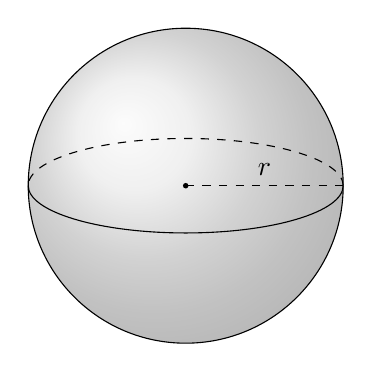
\begin{tikzpicture}
	\shade[ball color = gray!40, opacity = 0.4] (0,0) circle (2cm);
	\draw (0,0) circle (2cm);
	\draw (-2,0) arc (180:360:2 and 0.6);
	\draw[dashed] (2,0) arc (0:180:2 and 0.6);
	\fill[fill=black] (0,0) circle (1pt);
	\draw[dashed] (0,0 ) -- node[above]{$r$} (2,0);
	\end{tikzpicture}
	\captionof{figure}{Beispiel f\"ur $B(x,r)$ f\"ur $x\in\R^3$}
\end{center}
\end{Bemerkung}


\begin{Definition}(globaler Minimalpunkt)~ \\
	Ein Punkt $x^\ast\in\F$ hei\ss t \textbf{globaler Minimalpunkt} von $f$ auf $\F$ oder \textbf{globale L\"osung} von \eqref{eq:P}, falls 
	\begin{equation*}
	f(x)\geq f(x^\ast) \qquad \forall x\in\F 
	\end{equation*}
	gibt. \vspace{5pt}\\
	Ein Punkt $x^\ast\in\F$ hei\ss t \textbf{strikter globaler Minimalpunkt} von $f$ auf $\F$ oder \textbf{strikte globale L\"osung} von \eqref{eq:P}, falls 
	\begin{equation*}
	f(x)> f(x^\ast) \qquad \forall x\in\F ,\; x\neq x^\ast
	\end{equation*}
	gibt.
\end{Definition}

\paragraph{Einfache Beispiele}

\begin{enumerate}[label=\emph{\alph*})]
	\setcounter{enumi}{5}
	\item Die Funktion $f(x)=\sin(x)$ hat unendlich viele globale Minima.
	\item  Die Funktion
		\begin{equation*}
			f(x_1,x_2)=\frac{1}{2}(x_1^2+x_2^2)-\cos(x_1^2)-\cos(x_2^2)
		\end{equation*}
		hat ein striktes globales Minimum und noch weitere strikte lokale Minima. Die Funktion besteht aus einem quadratischen Term und noch zwei weiteren Termen, die man als \glqq Rauschen\grqq ~ interpretieren kann.
\end{enumerate}

\paragraph{Maximierung}

\begin{itemize}
	\item Oft soll die Zielfunktion $f$ maximiert werden, d.\,h., wir suchen ein $x^\ast \in \F$ mit
	\begin{equation*}
		f(x)\leq f(x^\ast) \qquad \forall x\in\F
	\end{equation*}
	\item Diese Aufgabe ist \"aquivalent dazu, ein $x^\ast\in\F$ zu finden mit
	\begin{equation*}
		-f(x)\geq -f(x^\ast)\qquad \forall x\in\F
	\end{equation*}
	\item[$\Rightarrow$] Äquivalentes Problem:
	\begin{gather}
	\label{eq:PMax}   
	\tag{PMax}
	\begin{aligned}
	\min 
	& & & g(x)=-f(x)\\
	\text{s.t.}
	& & & x\in\F
	\end{aligned}
	\end{gather}
	\item  Es gen\"ugt daher, nur Minimierungsaufgaben zu betrachten.
\end{itemize}
	
\section{Beispiele}
	\paragraph{Portfolio-Optimierung}
	\begin{itemize}
		\item Variablen: Aufteilung des Portfolios
		\item Nebenbedingungen: Budget, Beschr\"ankungen bei Investitionen
		\item Zielfunktion: maximale Rendite, minimales Risiko
	\end{itemize}
	\paragraph{Optimale Steuerung eines Raketenautos}
	\begin{itemize}
		\item Variablen: Beschleunigung des Autos
		\item Nebenbedingungen: Dynamik, maximale Beschleunigung
		\item Zielfunktion: Zielort erreichen, Verbrauch an Treibstoff minimieren
	\end{itemize}
	\paragraph{Data Fitting}
	\begin{itemize}
		\item Variablen: Modell-Parameter
		\item Nebenbedingungen: geg.\ Informationen, Parameterbeschr\"ankungen
		\item Zielfunktion: Abweichung/Fehler minimieren
	\end{itemize}
	
\subsection{Portfolio-Optimierung}
\begin{itemize}
	\item Es werden $n$ Wertpapiere gehandelt, wobei $R_j$ die Rendite des $j-$ten Wertpapiers in der n\"achsten Zeitperiode darstellt (\textbf{Zufallsvariable}).
	\item Ein \textbf{Portfolio} besteht aus einer Zusammenstellung dieser Wertpapiere, dargestellt durch nichtnegative Zahlen $x_j\in\R^+,j=1,\dots,n$.
	\item Rendite eines gegebenen Portfolios und die erwartete Rendite:
	\begin{equation*}
		R=\sum\limits_{j=1}^n x_jRj \qquad \mathbb{E}[R]=\sum\limits_{j=1}^n x_j\mathbb{E}[R_j]
	\end{equation*}
	\item Als Ma\ss{}  f\"ur das Risiko nutzen wir die durchschnittliche absolute Abweichung vom Erwartungswert
	\begin{equation*}
		\mathbb{E}[R-\mathbb{E}[R]]=\mathbb{E}\Bigg\lvert\sum\limits_{j=1}^n x_j (R_j-\mathbb{E}[R_j])\Bigg\rvert
	\end{equation*}
\end{itemize}
Es ergibt sich folgendes Optimierungsproblem:
\begin{eqnarray*}
		\max_{x_1,\dots,x_n} & &\mu\sum\limits_{j=1}^nx_j \mathbb{E}[R_j] - \mathbb{E}\Bigg\lvert\sum\limits_{j=1}^n x_j (R_j-\mathbb{E}[R_j])\Bigg\rvert\\
		\text{s.t.} & & \sum\limits_{j=1}^n x_j = 1\\
		& & x_j \geq 0, \qquad j=1,2,\dots,n
\end{eqnarray*}

\begin{itemize}
	\item Die beiden gegens\"atzlichen Ziele (erwartete Rendite maximieren vs. Risiko minimieren) werden durch den Parameter $\mu$ gewichtet
	\item Approximieren wir $\mathbb{E}[R_j]$ durch den Mittelwert der letzten beobachteten Renditen, l\"asst sich dieses Problem in ein \textbf{lineares Optimierungsproblem} transformieren
\end{itemize}

\subsection{Optimale Steuerung - Raketenauto}
Wir betrachten ein Auto mit Raketenantrieb, dass nur geradeaus f\"ahrt. Durch den Schub der Rakete kann das Auto sowohl nach links als auch nach rechts beschleunigen. Vom Startpunkt $x_0$ aus soll ein Ziel $x_f$ m\"oglichst genau in gegebener Zeit $t_f$ erreicht werden.
  
\begin{center}
    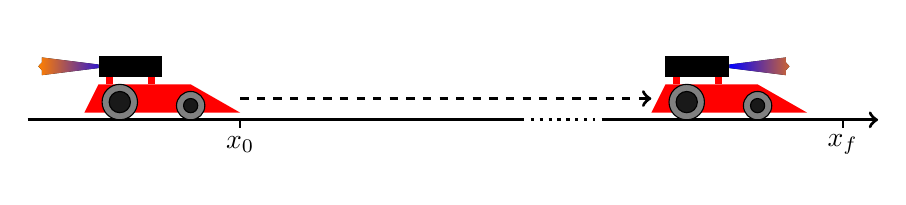
\begin{tikzpicture}[scale=0.9]
       \useasboundingbox (-3,-0.8) rectangle (9,1.3);
       % x-Achse
       \draw[very thick] (-3,0) -- (4,0);
       \draw[very thick,dotted] (4.1,0) -- (5.0,0);
       \draw[very thick,->] (5.1,0) -- (9,0);
       \draw[thick] (0,0) -- (0,-0.12); \draw (0,-0.35) node {$x_0$};
       \draw[thick] (8.5,0) -- (8.5,-0.12); \draw (8.5,-0.35) node {$x_f$};
       % Duesenauto, Karosserie
       \fill[red] (-2.2,0.1) -- (0,0.1) -- (-0.7,0.5) -- (-2,0.5);
       % Duesenauto, Raeder
       \draw[fill=black!50] (-0.7,0.2) circle (0.2);
       \draw[fill=black!90] (-0.7,0.2) circle (0.1);
       \draw[fill=black!50] (-1.7,0.25) circle (0.25);
       \draw[fill=black!90] (-1.7,0.25) circle (0.15);
       % Duesenauto, Duese
       \fill[red] (-1.2,0.5) -- (-1.2,0.6) -- (-1.3,0.6) -- (-1.3,0.5);
       \fill[red] (-1.8,0.5) -- (-1.8,0.6) -- (-1.9,0.6) -- (-1.9,0.5);
       \fill[black] (-2,0.6) -- (-1.1,0.6) -- (-1.1,0.9) -- (-2,0.9);
       % Duesenauto, Duesenstrahl
 	  \fill[left color=orange, right color=orange!20!blue] (-2,0.78) -- (-2,0.73) -- 
         (-2.8,0.63) -- (-2.8,0.70) -- (-2.85,0.755) --(-2.8,0.81) -- (-2.8,0.88) -- (-2,0.78);
       %
       \draw[very thick,->,dashed] (0,0.3) -- (5.8,0.3);
       %
       % Duesenauto, Karosserie
       \fill[red] (5.8,0.1) -- (8,0.1) -- (7.3,0.5) -- (6,0.5);
       % Duesenauto, Raeder
       \draw[fill=black!50] (7.3,0.2) circle (0.2);
       \draw[fill=black!90] (7.3,0.2) circle (0.1);
       \draw[fill=black!50] (6.3,0.25) circle (0.25);
       \draw[fill=black!90] (6.3,0.25) circle (0.15);
       % Duesenauto, Duese
       \fill[red] (6.8,0.5) -- (6.8,0.6) -- (6.7,0.6) -- (6.7,0.5);
       \fill[red] (6.2,0.5) -- (6.2,0.6) -- (6.1,0.6) -- (6.1,0.5);
       \fill[black] (6,0.6) -- (6.9,0.6) -- (6.9,0.9) -- (6,0.9);
       % Duesenauto, Duesenstrahl
 	  \fill[left color=blue, right color=blue!20!orange] (6.9,0.78) -- (6.9,0.73) -- 
         (7.7,0.63) -- (7.7,0.70) -- (7.75,0.755) --(7.7,0.81) -- (7.7,0.88) -- (6.9,0.78);
    \end{tikzpicture}
    \captionof{figure}{Düsenauto}
\end{center}
Starten wir am Punkt $(x_1(0),x_2(0)=(a_1,a_2)$ und wollen den Punkt $(0,0)$ so gut wie m\"oglich erreichen und zus\"atzlich den Energieverbrauch minimal halten, dann ergibt sich folgendes Optimierungsproblem:
\begin{eqnarray*}
		\min_{x_1,x_2,u} & & x_1(t_f)^2+x_2(t_f)^2+\alpha\int_{0}^{t_f}u(t)^2dt\\
		\text{s.t.} & & \dot{x_1}(t) = x_2(t)  \quad \dot{x_2}(t)=u(t),\\
		& & x_1(0)=a_1, \quad x_2(0)=a_2,\\
		& & b_l\leq u(t) \leq b_u \quad \text{f\"ur fast alle }t\in\left[0,t_f\right].
\end{eqnarray*}
Der Regularisierungsparameter $\alpha$ gewichtet hier zum einen die beiden Optimierungsziele, zum anderen gl\"attet er die optimale Steuerung. Gel\"ost wird diese Optimierungsproblem numerisch, indem man die Steuerung st\"uckweise konstant approximiert und die gew\"ohnlichen Differentialgleichungen der Nebenbedingungen mit dem Euler-Verfahren diskretisiert. Man erh\"alt hierbei ein \textbf{linear-quadratisches Optimierungsproblem}.
	
\begin{center}
     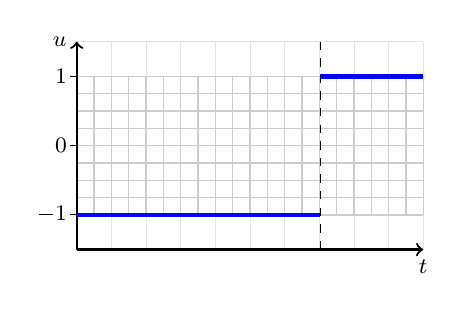
\begin{tikzpicture}[scale=0.88]
       \draw[draw=black!10,line width=0.25] (0,-1.5) grid[step=0.5] (5,1.5);
       \draw[draw=black!20,line width=0.5] (0,-1) grid[step=0.25] (5,1);
       \draw[thick,->] (0,-1.5) -- (5,-1.5) node[below] {\footnotesize{$t$}};
       \draw[thick,->] (0,-1.5) -- (0,1.5) node[left] {\footnotesize{$u$}};
       \foreach \u in {-1,0,1} {
         \draw (0,\u) node[left] {\footnotesize{$\u$}};
         \draw (-0.1,\u) -- (0,\u);
       }
       % Steuerung u
       \draw[ultra thick,blue] plot[domain=0:3.5174292] (\x,-1);
       \draw[ultra thick,blue] plot[domain=3.5174292:5] (\x,1);
       \draw[dashed] plot coordinates {(3.5174292,1.5) (3.5174292,-1.5)};
     \end{tikzpicture}
     %
     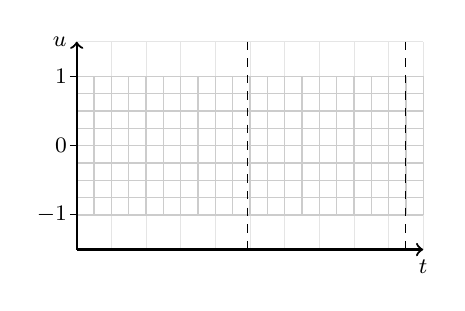
\begin{tikzpicture}[scale=0.88]
       \draw[draw=black!10,line width=0.25] (0,-1.5) grid[step=0.5] (5,1.5);
       \draw[draw=black!20,line width=0.5] (0,-1) grid[step=0.25] (5,1);
       \draw[thick,->] (0,-1.5) -- (5,-1.5) node[below] {\footnotesize{$t$}};
       \draw[thick,->] (0,-1.5) -- (0,1.5) node[left] {\footnotesize{$u$}};
       \foreach \u in {-1,0,1} {
         \draw (0,\u) node[left] {\footnotesize{$\u$}};
         \draw (-0.1,\u) -- (0,\u);
       }
       % Steuerung u
       \draw[blue,ultra thick] plot file {data/datenualpha.txt};
       \draw[dashed] plot coordinates {(2.4700,1.5) (2.4700,-1.5)};
       \draw[dashed] plot coordinates {(4.7500,1.5) (4.7500,-1.5)};
     \end{tikzpicture}
     \captionof{figure}{Optimale Steuerung f\"ur $\alpha = 0$ (links) und $\alpha = 1$ (rechts)}
\end{center}

\subsection{Lineare Regression}
Gegeben seien Messwerte $(\xi_i,\eta_i), i=1,\dots,m$. Der funktionale Zusammenhang zwischen den $\xi-$ und den $\eta-$ Werten soll durch eine Gerade
\begin{equation*}
	\eta(\xi)=g(\xi;x_1,x_2)= x_1\xi+x_2
\end{equation*}
beschrieben werden. Aufgrund von Messfehlern liegen nicht alle Messwerte auf der Geraden. Ziel ist es den Parameter $x=(x_1,x_2)\tr\in\R^2$ so zu bestimmen, dass die zugeh\"orige Gerade {\glqq optimal\grqq} zu den Messwerten passt.
   \begin{center}
     \begin{tikzpicture}
       \draw[->,thick] (0,0) -- (7,0) node[below]{$\xi$};
       \draw[->,thick] (1,0) -- (0,0) -- (0,5) node[left]{$\eta$};
       \draw (1,1) node{$\circ$} node[below right]{\footnotesize{$(\xi_1, \eta_1)$}};
       \draw (2.5,2) node{$\circ$} node[above left]{\footnotesize{$(\xi_2, \eta_2)$}};
       \draw (4,2.4) node{$\circ$} node[below right]{\footnotesize{$(\xi_3, \eta_3)$}};
       \draw (6,3.7) node{$\circ$} node[above left]{\footnotesize{$(\xi_4, \eta_4)$}};
       \draw[thick,red] (0,0.7) -- (7,4) node[below right]{$g(\xi; x_1, x_2)$};
     \end{tikzpicture}
     \captionof{figure}{Lineare Regression}
   \end{center}
Das \"ubliche Kriterium f\"ur Optimalit\"at ist die Minimierung der Summe der Fehlerquadrate in den Messpunkten. Dazu definieren wir die Zielfunktion $f: \R^2 \to \R$ durch
\begin{equation*}
	f(x)= \sum\limits_{i=1}^m\left[g(\xi_i,x) - \eta_i \right]^2 = \sum\limits_{i=1}^m\left[x_1\xi_i+x_2-\eta_i \right]^2
\end{equation*}
Das resultierende Optimierungsproblem
\begin{equation*}
	\min_{x_1,x_2}\sum\limits_{i=1}^m\left[x_1\xi_i+x_2-\eta_i \right]^2
\end{equation*}
ist \textbf{unrestringiert} und die Zielfunktion ist \textbf{quadratisch}.
\newpage

%%%%%%%%%%%%%%%%%%%%%%%%%%%%%%%%%%%%%%%%%%%%%
\chapter{Konvexe Optimierungsprobleme}
%%%%%%%%%%%%%%%%%%%%%%%%%%%%%%%%%%%%%%%%%%%%%

\begin{itemize}
\item Historisch standen lineare Probleme im Fokus der Optimierung.
\item Urspr\"ungliche Unterscheidung in lineare und nichtlineare Probleme.
\item  Aber: Bestimmte nichtlineare Probleme k\"onnen effizient gel\"ost werden.
\item  Daher unterscheidet man zwischen \textbf{konvexen und nichtkonvexen Problemen}.
\end{itemize}
Das auf Seite \pageref{eq:P} vorgestellte Problem \eqref{eq:P}
\begin{gather}
\tag{P}
\begin{aligned}
\min_x
& & & f(x) \\
\text{s.t.}
& & & x\in \mathcal{F}
\end{aligned}
\end{gather}
ist genau dann ein \textbf{konvexes Optimierungsproblem}, wenn die zul\"assige Menge $\F$ konvex ist und die Zielfunktion $f$ konvex auf $\F$ ist.

\paragraph{Probleme mit Gleichungs- und Ungleichungsrestriktionen}~\\

Typischerweise ist die zul\"assige Menge durch Gleichungen und Ungleichungen definiert.
Das Problem
 \begin{gather}
   \label{eq:QP}   
   \tag{QP}
   \begin{aligned}
     \min_x
     & & & f(x) \\
     \text{s.t.}
     & & & h_i(x) = 0\,, \quad i = 1,\ldots,m\,,\\
     & & & g_j(x) \leq 0\,, \quad j = 1,\ldots,p\,.
   \end{aligned}
 \end{gather}
ist konvex, wenn $f$ und $g_j,j=1,\dots,p$ konvexe Funktionen sind, und die Funktionen $h_i,i=1,\dots,m$ affin-linear sind, d.h.,
\begin{equation*}
	h_i(x)=a_i\tr x+b_i,\qquad i=1,\dots,m,
\end{equation*}
mit $a_i\in\R^n$ und $b_i\in\R$.

\section{Konvexe Mengen}

\begin{Definition}(konvexe Menge)\\
	Eine Menge $C\subseteq\R^n$ hei\ss t konvex, falls f\"ur beliebige $x,y\in C$ gilt
	\begin{equation*}
	\lbrace (1-t)x+ty ~\vert~ 0\leq t \leq 1\rbrace  \subseteq C
	\end{equation*}
	d.h., f\"ur die Verbindungsstrecke $\left[x,y\right]=\{(1-t)x+ty ~\vert~ 0\leq t \leq 1 \}$ gilt $\left[x,y\right]\subseteq C$.
\end{Definition}
\begin{center}
	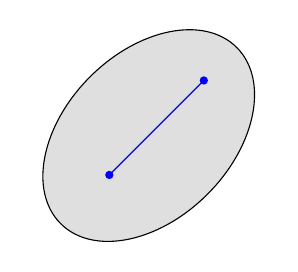
\begin{tikzpicture}
	\draw[rotate=-45,fill=gray!25] (0,0) ellipse (30pt and 45pt);
	\textcolor{blue}{
		\draw (-0.5,-0.5) -- (0.7,0.7);
		\fill (-0.5,-0.5) circle[radius=1.5pt];
		\fill (0.7,0.7) circle[radius=1.5pt];
	}
	%\draw (-0.7,0.6) node[below] {\Large $C$};
	\end{tikzpicture}
	\qquad \qquad
	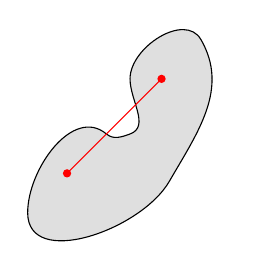
\begin{tikzpicture}
	\useasboundingbox (-1,-1.35) rectangle (1.5,1.35);
	\draw[fill=gray!25] (0,0) to [out=140,in=90] (-1,-1)
	to [out=-90,in=240] (0.8,-0.6)
	to [out=60,in=-60] (1.2,1.2)
	to [out=120,in=90] (0.3,0.7)
	to [out=-90,in=20] (0.3,0)
	to [out=200,in=-40] (0,0);
	\textcolor{red}{
		\draw (-0.5,-0.5) -- (0.7,0.7);
		\fill (-0.5,-0.5) circle[radius=1.5pt];
		\fill (0.7,0.7) circle[radius=1.5pt];
	}
	%\draw (0.3,-0.2) node[below] {\Large $N$};
	\end{tikzpicture}
	\captionof{figure}{links: konvexe Menge, rechts: keine konvexe Menge}
\end{center}


%\begin{Satz}
%F\"ur eine konvexe Optimierungsaufgabe ist jede lokale L\"osung eine globale L\"osung, und die L\"osungsmenge von \eqref{eq:QP}
%\begin{equation*}
%	\mathcal{S}=\{ x\in\F ~\vert~ f(x)\leq f(y~\forall y\in\F)\}
%\end{equation*}
%ist konvex.
%\end{Satz}
%\begin{proof}
%Sp\"ater in der Vorlesung
%\end{proof}
%\begin{Bemerkung}
%	Über die \textbf{Existenz einer L\"osung} haben wir hier noch keine Aussage getroffen!
%\end{Bemerkung}


\subsection{Beispiele}
\begin{enumerate}[label=\emph{\alph*})]
	\item Die konvexen Teilmengen des $\R$ sind, neben $\R$ selbst, die Intervalle. Beispielsweise $\left[a,b \right]$ mit $a,b\in\R,a\leq b,$ oder $\left]a,\infty\right[$ mit $a\in\R$.
	\begin{proof}
	$C=\left[a,b \right]$ mit $a,b\in\R,~a\leq b \Rightarrow C$ ist konvex.\\
	Seien $x,y ~\text{beliebige Punkte aus } C \text{ und } t\in\left[0,1 \right]$. Dann gilt einerseits die Absch\"atzung nach unten
	\begin{equation*}
		(1-t)x+ty \stackrel{a \leq x,y}{\geq} (1-t)a+ta = a
	\end{equation*}
	 und andererseits die Absch\"atzung nach oben durch 
	 \begin{equation*}
		(1-t)x+ty \stackrel{x,y\leq b}{\leq} (1-t)b-tb=b
	 \end{equation*}
	 Das hei\ss t zu zwei beliebigen Punkten $x,y$ aus dem Intervall $\left[a,b \right]$ liegt das davon erzeugte Teilintervall $\left[x,y\right]\subseteq \left[a,b\right]$.
	\end{proof}
	\item F\"ur $x\in\R^n$ und $r>0$ bezeichnen wir mit
	\begin{equation*}
		B(x,r)=\lbrace y\in\R^n ~\vert~ \norm{y-x} <r\rbrace
	\end{equation*}
	die offene Kugel und mit
		\begin{equation*}
	\bar{B}(x,r)=\lbrace y\in\R^n ~\vert~ \norm{y-x} \leq r\rbrace
	\end{equation*}
	die abgeschlossene Kugel mit Radius $r$ um den Punkt $x$. Beide Mengen sind konvex.\footnote{siehe Übungsblatt 1}
	\item Hyperebenen
	\begin{equation*}
		\mathcal{H}(a,b)=\lbrace x\in\R^n ~\vert~ a\tr x=b \rbrace
	\end{equation*}
	mit $a\in\R^n,b\in \R$ und die durch sie definierten Halbr\"aume $\lbrace x\in\R ~\vert~ a\tr x\leq b \rbrace$ sind konvexe Mengen.
	\item Polyeder
	\begin{equation*}
	P(A,b)=\lbrace x\in\R^n ~\vert~ Ax\leq b \rbrace
	\end{equation*}
	mit $A\in\R^{m\times n}$ und $b\in\R^m$ sind konvex.
	\begin{proof}
	Seien $x_1,x_2\in P(A,b)$ und $t\in\left[0,1\right]$ $\Rightarrow Ax_1\leq b \wedge Ax_2\leq b$.\\ Dann gilt
	\begin{eqnarray*}
		A\left[(1-t)x_1+tx_2 \right] & = & A(1-t)x_1+A(tx_2)\\
									& = & (1-t)\underbrace{Ax_1}_{\geq b}+t\underbrace{Ax_2}_{\leq b}\\
									& \leq & (1-t)b + tb =b\\
									& \Leftrightarrow & (1-t)x_1+tx_2 \in P(A,b)
	\end{eqnarray*}
	\end{proof}
	\begin{Bemerkung}
		Ein typischer Fall einer zul\"assigen Menge beschrieben durch Gleichungen und Ungleichungen, ist gegeben durch
		\begin{equation*}
			\bar{P}(A,b,G,r) = \lbrace x\in \R^n ~\vert~ Ax\leq b~,~Gx=r\rbrace
		\end{equation*}
		Wie kann man zeigen, dass diese Menge konvex ist?
		Es gilt:
		\begin{equation*}
			Gx=r \Leftrightarrow \left( Gx\leq r \right) \wedge ( \underbrace{Gx\geq r}_{-Gx\leq -r})
		\end{equation*}
		Damit ist
		 \begin{equation*}
			\Rightarrow \begin{bmatrix}&A\\&G\\-&G\end{bmatrix}x\leq \begin{bmatrix}&b\\&r\\-&r
			\end{bmatrix}
		 \end{equation*} 
		 ein Spezialfall von oben.
	\end{Bemerkung}
\end{enumerate}
\subsection{Schnitt, Skalierung und Verschiebung}
\begin{Lemma}Ist $\left(C_j \right)_{j\in J}$ eine Familie konvexer Mengen mit einer beliebigen Indexmenge $J$, dann ist auch $C=\bigcap\limits_{j\in J} C_j$ konvex.
\end{Lemma}
\begin{proof}
	Folgt unmittelbar aus der Definition.
\end{proof}

\begin{Lemma}
	Ist $C\subseteq \R^n$ konvex, dann ist auch
	\begin{equation*}
		aC + b = \lbrace ax+b ~\vert~ x\in C \rbrace
	\end{equation*}
	konvex f\"ur alle $a\in\R$ und $b\in\R^n$.
\end{Lemma}

\begin{Definition}(Konvexkombination)\\
	Sind $x^{(1)},\dots,x^{(k)}\in\R^n$ und $\alpha_1,\dots\alpha_k \in\R$, dann hei\ss t ein Vektor
	\begin{equation*}
		\sum\limits_{i=1}^k\alpha_ix^{(i)}~ \text{mit} ~ \sum\limits_{i=1}^k \alpha_i = 1~ \text{und} ~ \alpha_i\geq 0, i=1,\dots,k,
	\end{equation*}
	Konvexkombination der Vektoren $x^{(1)},\dots,x^{(k)}$.
\end{Definition}
\begin{Satz}
Eine Menge $C\subset\R^n$ ist genau dann konvex, wenn sie alle Konvexkombinationen von Punkten in $C$ enth\"alt.
\end{Satz}
\begin{proof} siehe Übungsblatt 1
\end{proof}

\begin{Definition}(Konvexe H\"ulle)\\
	F\"ur $A\subset\R^n$ ist die konvexe H\"ulle von $A$, bezeichnet mit $\co A$, die kleinste konvexe Menge, die $A$ umfasst, d.h.
	\begin{equation*}
		\co A = \bigcap\lbrace C\subseteq \R^n ~\vert~ C~\text{konvex}, C\supseteq A \rbrace
	\end{equation*}
\end{Definition}
\begin{Lemma}
	F\"ur $A\subset\R^n$ ist
	\begin{equation*}
		\co A = \lbrace x\in \R^n ~\vert~ x ~\text{ist Konvexkombination von Punkten in }A\rbrace.
	\end{equation*}
\end{Lemma}
\begin{proof}~\\
	Sei $B=\lbrace x\in\R^n ~\vert~ x \text{ ist Konvexkombination von Punkten in } A \rbrace \underbrace{\Rightarrow}_{\text{z.z.}} \co A = B$\\
	$B$ konvex und $A\subseteq B \Rightarrow \co A \subseteq \co B = B$.\\
	Umgekehrt gilt $\forall C$ konvex mit $C\supseteq A \Rightarrow C\supseteq B \underbrace{\Rightarrow}_{C=\co A} \co A \supseteq B$
\end{proof}
\begin{Definition}(Kegel)~\\
	Eine nichtleere Menge $K\subseteq\R^n$ hei\ss t \textbf{Kegel}, wenn mit $x\in K$ auch $tx\in K$ f\"ur alle $t>0$ gilt, d.h., wenn mit $x\in K$ auch der offene Halbstrahl $\lbrace tx ~\vert~ t>0\rbrace\subseteq K$ ist.
\end{Definition}

\begin{Lemma}
	Ein Kegel $K\subseteq \R^n$ ist genau dann konvex, wenn $K+K\subseteq K$ ist.
\end{Lemma}
\begin{proof}
	s. Übungsblatt 1
\end{proof}

\paragraph{Beispiele f\"ur Kegel}

\begin{enumerate}[label=\emph{\alph*})]
	\item Der Kegel $\lbrace x\in\R^n ~\vert~ x \geq 0_n \rbrace$ ist konvex. Es gilt $K+K=K$.
	\item Die Menge
	\begin{equation*}
		\lbrace x\in\R^n~\vert~x\geq 0_n \rbrace\cup\lbrace x\in\R^n~\vert~x\leq 0_n \rbrace
	\end{equation*}
	ist ein Kegel, aber nicht konvex, denn es gilt $K+K= \R^n\not\subseteq K$.
	\item Der Kegel der positiv semidefiniten Matrizen
	\begin{equation*}
		\mathcal{S}^n_+=\lbrace X\in\mathcal{S} ~\vert~ X\succcurlyeq 0\rbrace
	\end{equation*}
	ist konvex, wobei $\mathcal{S}^n$ die Menge der symmetrischen $n \times n$-Matrizen ist.
\end{enumerate}

\paragraph{Wichtige Kegel}

\begin{Definition}
 Ist $S\subseteq \R^n$ und $x\in S$, dann hei\ss t die Menge
 \begin{equation*}
 	K(S,x)=\lbrace t(s-x) ~\vert~ s\in S, ~t>0  \rbrace
 \end{equation*}
 der von $S-x$ ~\textbf{erzeugte Kegel} oder \textbf{konische H\"ulle} von $S-x$.
\end{Definition}
Die Menge $K(S,x)$ besteht aus Halbstrahlen, die durch die Vektoren $S-x$ erzeugt werden, s.d. die Menge nach Definition ein Kegel ist. Wegen $x\in S$ ist immer  auch $0_n\in K(S,x)$ (f\"ur $s=x$) und es gilt $K(S,x)=K(s-x,0_n)$.

\begin{Lemma}
	Sei $C\subseteq \R^n$ konvex und $x\in C$. Dann ist $K(C,x)$ konvex.
\end{Lemma}
\begin{proof}
	cf. undergraduate convexity
\end{proof}
\begin{Definition}
	Ist $C\subseteq\R^n$ konvex und $x\in C$. Dann hei\ss t $s\in\R^n$ \textbf{Normalenrichtung} von $C$ in $x$, wenn 
	\begin{equation*}
		\langle s,y-x \rangle \leq 0 \qquad \forall y\in C
	\end{equation*}
	gilt. Die Menge
	\begin{equation*}
		N(C,x) = \lbrace s\in R^n ~\vert~ s \, \text{ist Normalenrichtung von $C$ in $x$} \rbrace
	\end{equation*}
	hei\ss t \textbf{Normalenkegel} von $C$ in $x$.
\end{Definition}
\begin{Bemerkung}
	Der Normalenkegel ist konvex und abgeschlossen.
\end{Bemerkung}
Ein Beispiel f"ur einen Normalenkegel l"asst sich wie folgt konstruieren.
Seien $C$ ein Unterraum und $x \in C$ beliebig.
Dann ist die konische H"ulle $K(C,x) = C$ und der Normalenkegel $N(C,x) = C^\bot$, also das orthogonale Komplement von $C$.
Der Beweis der Aussage ist eine gute "Ubung.
%
\section{Konvexe Funktionen}

\begin{Definition}(konvexe Funktion)\\
	Ist $D\subseteq \R^n$ und ist $\emptyset \neq C\subseteq D$ konvex, dann hei\ss t die Funktion $f\colon D\to\R$ konvex auf $C$, wenn
	\begin{equation*}
		f((1-t)x+ty)\leq(1-t)f(x)+tf(y)
	\end{equation*}
	f\"ur alle $x,y\in C$ und alle $t\in\left[0,1 \right]$ gilt.
\end{Definition}

\begin{Definition}[Epigraph]
\label{def:epi}
 Der \emph{Epigraph} einer Funktion $f : \R^n \to \R$ ist definiert als
 \begin{equation*}
 	\lbrace (x, r)^T \, \vert \, x \in D, r \geq f(x) \rbrace \subseteq \R^{n + 1} =: \text{epi}\, f\qedhere
 \end{equation*}
\end{Definition}
\begin{Bemerkung}[Epigraphcharakterisierung von Funktionen]
	Die obige Definition erlaubt uns nun eine konvexe Funktion als eine Funktion aufzufassen, deren Epigraph eine konvexe Menge ist.
	In der Tat lassen sich die meisten Klassen von Funktionen, die in der Optimierung eine Rolle spielen, durch "aquivalente Charakterisierungen des Epigraphen in Mengensprache fassen.
\end{Bemerkung}
\begin{Definition}[strikte und gleichm"a"sige Konvexit"at]
\label{def:str-convty}
 Gilt f"ur eine Funktion $f \colon \R^n \to \R$
 \begin{equation*}
 	\forall t \in (0, 1) \forall x,y \in D : f((1 - t)x + ty) < (1 - t)f(x) + tf(y)
 \end{equation*}
 so sprechen wir von einer \emph{stikt}, \emph{streng} oder \emph{stark} konvexen Funktion.
 Gilt au"serdem auch
 \begin{equation*}
 	\forall t \in (0, 1) \forall x,y \in D : f((1 - t)x + ty) + \frac{\lambda}{2}\Vert x \Vert^2_2 \leq (1 - t)f(x) + tf(y)
 \end{equation*}
 so sprechen wir auch von einer \emph{gleichm"a"sig} konvexen Funktion zum Parameter $\lambda$. 
\end{Definition}
\begin{Bemerkung}
	Wenn die beiden Konzepte verbal formulieren wollen, so bedeutet \emph{strikt} konvex, dass eine Funktion superlinear gekr"ummt ist.
	\emph{Gleichm"a"sige} Konvexit"at bedeutet dann, dass die Kr"ummung von $f$ mindestens quadratisch ist.
	In der Tat gilt
	\begin{equation*}
		\text{glm. Konvexit"at} \Rightarrow \text{strikte Konvexit"at} \Rightarrow \text{Konvexit"at}
	\end{equation*}
	w"ahrend keine der Umkehrungen gilt.
\end{Bemerkung}

\paragraph{Beispiele konvexer Funktionen}

\begin{enumerate}[label=\emph{\alph*})]
	\item $f(x) = x$ ist konvex auf $\R$, ebenso auch $-f(x)$ und $f$ damit ebenfalls konkav.
	\item $f(x) = x^2$ ist sogar strikt konvex auf $\R$ %nach foliendef sogar glm conv
	\item $f(x) = x^3$ ist nicht konvex auf $\R$ aber gleichm"a"sig konvex auf $C = [0, \infty)$
	\item $f(x) = \exp(\alpha x)$ ist f"ur alle $\alpha$ konvex auf $\R$
	\item $f(x) = -\log(x)$ ist strikt konvex auf $(0, \infty)$
	\item Eine beliebige Norm $\Vert\cdot\Vert$ auf $\R^n$ ist konvex, aber nicht strikt konvex ("Ubungsblatt 1)
	\item Die $\max$-Funktion $f(x) = \max \lbrace x_1, \ldots, x_n \rbrace$ ist konvex auf $\R^n$
\end{enumerate}
%begin characterisations of convex functions
\subsection{Charakterisierungen konvexer Funktionen}
Wir betrachten nun ausreichend sch"one Funktionen, d.\,h., Funktionen f"ur die die Voraussetzungen der folgenden Theoreme gegeben sind.
Dazu z"ahlen insbesondere die differenzierbaren und die stetig differenzierbaren Funktionen.
\begin{Satz}[Charakterisierung erster Ordnung]
\label{chr1O1}
	Seien $D\subseteq\R^n$ offen, $\emptyset\neq\F\subseteq D$ konvex und $f:D\to\R$ differenzierbar auf $D$.
	Dann ist $f$ auf $\F$ konvex genau dann, wenn $\forall x, y \in \F$ gilt:
	\begin{equation}
		f(y) \geq f(x) + \nabla f(x)\tr(y - x)
	\end{equation}
\end{Satz}
%
\begin{Satz}[Charakterisierung erster Ordnung]
\label{chr1O2}
	Seien $D\subseteq\R^n$ offen, $\emptyset\neq\F\subseteq D$ konvex und $f:D\to\R$ differenzierbar auf $D$.
	Dann ist $f$ auf $\F$ strikt konvex genau dann, wenn $\forall x, y \in \F$ gilt:
	\begin{equation}
		f(y) > f(x) + \nabla f(x)\tr(y - x)
	\end{equation}
	\noindent
	Gilt au"serdem f"ur $\mu \in (0, \infty)$
	\begin{equation}
		f(y) - f(x) > \nabla f(x)\tr(y - x) + \mu\Vert y - x \Vert^2
	\end{equation}
	\noindent
	so hei"st $f$ gleichm"a"sig konvex.
\end{Satz}
%
\begin{Satz}[Charakterisierung zweiter Ordnung]
\label{thm:chr2O1}
	Seien $D\subseteq\R^n$ offen, $\emptyset\neq\F\subseteq D$ konvex und $f:D\to\R$ zweimal stetig differenzierbar auf $D$.
	Wenn $\forall x, y \in \F$ gilt:
	\begin{equation}
		\nabla^2 f(x) \succcurlyeq 0
	\end{equation}
	\noindent
	so ist $f$ konvex auf $\F$ und falls $\F$ offen ist, so gilt auch die Umkehrung.
\end{Satz}
%
\begin{Satz}[Charakterisierung zweiter Ordnung]
\label{thm:chr2O2}
	Seien $D\subseteq\R^n$ offen, $\emptyset\neq\F\subseteq D$ konvex und $f:D\to\R$ zweimal stetig differenzierbar auf $D$.
	Wenn $\forall x\in \F$ gilt:
	\begin{equation}
		\nabla^2 f(x) \succ 0
	\end{equation}
	\noindent
	also $\forall x \in \F$ und $0\neq d\in\R^n$
	\begin{equation}
		d\tr\nabla^2 f(x)d > 0
	\end{equation}

	\noindent
	so ist $f$ stikt konvex auf $\F$.
\end{Satz}
%
\begin{Bemerkung}
	Die Umkehrung von \ref{thm:chr2O2} gilt im Allgemeinen nicht.
\end{Bemerkung}
%
\begin{Satz}[Charakterisierung zweiter Ordnung]
\label{thm:chr2O3}
	Seien $D\subseteq\R^n$ offen, $\emptyset\neq\F\subseteq D$ konvex und $f:D\to\R$ zweimal stetig differenzierbar auf $D$.
	Ist $\nabla^2 f(x)$ gleichm"a"sig positiv definit, also wenn $\forall x \in \F$, $d\in\R^n$ und $\beta\in(0,\infty)$
	\begin{equation}
		d\tr\nabla^2 f(x)d > \beta \Vert d\Vert^2
	\end{equation}

	\noindent
	gilt, so ist $f$ gleichm"a"sig konvex auf $\F$. Ist $\F$ offen, so gilt auch die Umkehrung.
\end{Satz}
%
\paragraph{Rechenregeln f"ur konvexer Funktionen}


\begin{enumerate}[label=\emph{\alph*})]
	\item Seien $f_i, i\in[n]$ konvex und $\alpha_i\in\R$.
		  Dann ist auch $\sum_{i=1}^n\alpha_if_i$ konvex.
	\item Seien $f$ konvex, $A\in\R^{m\times n}$ und $b\in\R^m$.
		  Dann ist auch $g(x):=f(Ax+b)$ konvex.
	\item Seien $J$ eine beliebige auch unendliche Indexmenge und $f_j$ konvex f"ur alle $j\in J$.
		  Dann ist auch $\max_{j\in J}f_j(x)$ konvex.
	\item Seien $g(x,y)$ konvex in $x$ und $y$ und die Menge $C$ konvex.
		  Dann ist auch $f(x) := \min_{y\in C}g(x,y)$ konvex.
\end{enumerate}